% Shared preamble of the HSEMHS mode documents (docs/physics/*.tex, docs/technical/*.tex).
\documentclass[10pt]{extarticle}
\usepackage[a4paper,margin=1.7cm]{geometry}
\usepackage[T1]{fontenc}\usepackage{lmodern}\usepackage{tabularx}
\usepackage{amsmath,amssymb,bm,enumitem,titlesec,xcolor,booktabs,array,tikz,graphicx,longtable}
\usepackage[hidelinks]{hyperref}
\titleformat{\section}{\large\bfseries\color{blue!50!black}}{\thesection.}{0.5em}{}
\titlespacing*{\section}{0pt}{9pt}{3pt}
\titleformat{\subsection}{\normalsize\bfseries}{\thesubsection}{0.5em}{}
\titlespacing*{\subsection}{0pt}{6pt}{2pt}
\setlist{nosep,leftmargin=1.3em}
\setlength{\parindent}{0pt}\setlength{\parskip}{4pt}
\renewcommand{\arraystretch}{1.15}
\newcommand{\B}{\mathbf B}\newcommand{\J}{\mathbf J}\newcommand{\F}{\mathbf F}\newcommand{\R}{\mathbf R}
\newcommand{\zh}{\hat{\mathbf z}}\newcommand{\Bo}{\mathbf B_{\rm obs}}\newcommand{\Lv}{\mathbf L}
\newcommand{\code}[1]{\texttt{#1}}
\newcolumntype{L}[1]{>{\raggedright\arraybackslash}p{#1}}
\newcolumntype{Y}{>{\raggedright\arraybackslash}X}
\newcommand{\doctitle}[2]{{\Large\bfseries #1}\\[2pt]{\small #2}\par\vspace{2pt}}
\pagestyle{plain}
\AtBeginDocument{\sloppy}

\begin{document}
\doctitle{full-mhs-z: full magnetohydrostatic equilibrium on a height grid}{Physics of \code{run.mode = "full-mhs-z"} (HSEMHS; the M5i configuration). 24 Oct 2026.}

\section{What the mode does}
It looks for a \textbf{static} magnetised atmosphere that stays as close as possible to the input: the temperature is
kept exactly, the magnetic field is allowed to change but is kept close to the input field $\Bo$, and the pressure
(hence the density) adjusts until the forces balance. Unlike the \code{mhs-poisson} modes, both $P$ and $\B$ change.
This is the only mode that can, in principle, remove the non-gradient part of the force imbalance (the buoyancy of the
temperature structure), because only a changed field can supply the magnetic tension it requires.

\section{Quantities}
\begin{tabular}{>{$}l<{$} p{11.0cm} l}
\toprule
\text{Symbol} & Meaning & Unit \\ \midrule
T & temperature from the input, \textbf{never changed} & K \\
P,\ u & gas pressure, unknown; $u=\ln P$ & Pa, -- \\
\B,\ \Bo & model magnetic field (unknown) and the input field & T \\
\mathbf A,\ \bar b & vector potential on cell edges and the mean vertical field: the field unknowns & T\,m, T \\
\J & current $\nabla\times\B/\mu_0$ & A\,m$^{-2}$ \\
\sigma & allowed deviation of $\B$ from $\Bo$; M5i: \textbf{uniform 5\,G} per component & T \\
S & local weight scale $\max(\rho_0g,\,0.01\,\mathrm{median}_{\rm layer}\rho_0g)$ from the starting state, fixed & N\,m$^{-3}$ \\
P_{\rm ref} & mean of $\ln P$ on the bottom plane (the gauge); production $5.22\times10^6$\,Pa at $-2.44$\,Mm & Pa \\
\bottomrule
\end{tabular}

\section{The equations}
\[
\boxed{\;-\nabla P+\J\times\B-\rho g\,\zh=0,\qquad\nabla\cdot\B=0\;}
\qquad \J\times\B=-\nabla\frac{B^2}{2\mu_0}+\frac{(\B\cdot\nabla)\B}{\mu_0}.
\]
The Lorentz force is a magnetic pressure plus a tension. Taking the curl, static balance needs
$\nabla\times(\J\times\B)=g(\partial_y\rho,-\partial_x\rho,0)$: wherever the density varies horizontally (hot and cool
gas side by side), the tension of the field must hold it up. A field taken from a moving simulation does not satisfy
this, so with $\B=\Bo$ fixed no pressure can make the atmosphere static. The mode therefore lets $\B$ change, by as
little as possible.

\section{The field on a staggered grid}
\begin{minipage}[t]{0.57\linewidth}\vspace{0pt}
$P$, $\rho$, $T$ live at cell centres. Each field component lives on the cell face it points through ($B_x$ on
$x$-faces, \dots), and the unknown is the vector potential $\mathbf A$ on the cell edges, with
\[
\B=\nabla\times\mathbf A+\bar b\,\zh .
\]
The discrete divergence of a discrete curl is identically zero, so \textbf{$\nabla\cdot\B=0$ holds exactly} and is never
enforced. $\bar b$ supplies the net vertical flux through the periodic box, which a curl cannot. Currents live on the
edges. Each force component is evaluated on the faces of its own direction, and only the other two field components
enter it (a field along $x$ exerts no force along $x$).
\end{minipage}\hfill
\begin{minipage}[t]{0.39\linewidth}\vspace{0pt}\centering
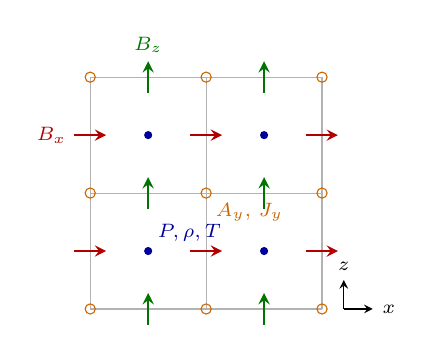
\begin{tikzpicture}[scale=0.92,>=stealth]
\draw[gray!60] (0,0) grid[step=1.6] (3.2,3.2);
\foreach \x in {0.8,2.4}\foreach \z in {0.8,2.4}{\fill[blue!60!black] (\x,\z) circle (1.6pt);}
\node[blue!60!black,font=\scriptsize,above right] at (0.8,0.8) {$P,\rho,T$};
\foreach \x in {0,1.6,3.2}\foreach \z in {0.8,2.4}{\draw[->,red!70!black,thick] (\x-0.22,\z)--(\x+0.22,\z);}
\node[red!70!black,font=\scriptsize,left] at (-0.2,2.4) {$B_x$};
\foreach \x in {0.8,2.4}\foreach \z in {0,1.6,3.2}{\draw[->,green!45!black,thick] (\x,\z-0.22)--(\x,\z+0.22);}
\node[green!45!black,font=\scriptsize,above] at (0.8,3.4) {$B_z$};
\foreach \x in {0,1.6,3.2}\foreach \z in {0,1.6,3.2}{\draw[orange!80!black] (\x,\z) circle (2pt);}
\node[orange!80!black,font=\scriptsize,below right] at (1.6,1.6) {$A_y,\,J_y$};
\draw[->] (3.5,0)--(3.9,0) node[right,font=\scriptsize]{$x$};
\draw[->] (3.5,0)--(3.5,0.4) node[above,font=\scriptsize]{$z$};
\end{tikzpicture}\\[-2pt]
{\scriptsize An $x$--$z$ slice of the staggered mesh.}
\end{minipage}

\section{The compromise that is minimised}
\[
\Phi=\underbrace{\lambda_F\Big\langle\frac{|\R|^2}{S^2}\Big\rangle_{\rm faces}}_{\Phi_F\ \text{forces}}
+\underbrace{\Big\langle\frac{(\B-\Bo)^2}{\sigma^2}\Big\rangle_{\rm faces}}_{\Phi_B\ \text{data}}
+\underbrace{\Phi_S}_{\text{smooth }\delta\B}+\underbrace{\Phi_Q}_{\text{no grid-scale currents}},
\qquad \R=\nabla P+\rho g\zh-\J\times\B .
\]
\begin{itemize}
\item $\Phi_F$: the force residual on every face in units of the local weight $S$; $|\R|/S=1$ means an unbalanced force
as large as gravity. $\lambda_F=10^{-4}$.
\item $\Phi_B$: each face compares its component with $\Bo$ interpolated to the face. $\Phi_B=1$ is a mean deviation of
one $\sigma$. With the M5i choice $\sigma=5$\,G uniform, any change of $\B$ costs the same everywhere: there is no relative
tolerance, because with real observations no meaningful $\sigma_B$ exists (Stokes noise does not translate into
field errors).
\item $\Phi_S$: second differences of $\delta\B=\B-\Bo$ (at centres, in units of $\sigma$) are penalised ($\lambda_S=10^{-3}$):
the correction must be smooth, not cell-to-cell noise.
\item $\Phi_Q$: second differences of the currents along the grid ($\lambda_Q=10^{-3}$, scaled by $\lambda_F$): the
field may not balance forces with zig-zag currents, which are numerical artefacts.
\end{itemize}
The temperature is fixed, so $\rho=\rho(T,P)$ and the opacity follow from $P$ alone.

\section{Boundary conditions and gauge}
Periodic in $x$ and $y$. The horizontal force equations are used on the interior layers only (the top and bottom
layers lack a vertical current term). The pressure level is fixed by the mean of $\ln P$ on the bottom plane
(\code{P\_ref} from the input file), not by a pressure map. Safety limits: in one step $\ln P$ changes by at most 5 at
any point, and $P$ never drops below $e^{-3}$ of its starting value.

\section{How the solution is reached}
\begin{enumerate}
\item \textbf{Pressure start:} each column in exact discrete hydrostatic equilibrium on the staggered mesh, from the
bottom pressure.
\item \textbf{Field start:} with the pressure frozen, $\mathbf A$ is fitted to $\Bo$ (data and smoothness terms only), a
linear least-squares problem.
\item \textbf{Joint Gauss--Newton:} linearise $\R$, solve the normal equations for a change of $(\ln P,\mathbf A,\bar b)$,
and accept it if $\Phi$ decreases. M5i: no trust radius; a rejected step is halved along the same direction
(backtracking line search).
\item \textbf{Stop} when $|\Delta\Phi|/\Phi<10^{-6}$ on three consecutive accepted steps (M5i uses $\Phi$ itself as the
convergence variable; the M5h variant used the height of $\tau=1$).
\end{enumerate}
After every accepted step the height of $\tau_{500}=1$ is recomputed in every column and recorded, since that is the
quantity spectral lines respond to.

\section{What to expect}
\begin{itemize}
\item The run is long: about $5\times10^8$ unknowns on the full cube ($504\times504\times496$). The M5i run of 22--23 Oct
used 24 ranks on 4 nodes; it reached $\Phi=7.9\times10^3$ after 112 accepted steps, when it was stopped on request (23 Oct). M5h (5\,\% relative $\sigma$, trust region) ran to its 24\,h wall limit.
\item In strong-field, low-$\beta$ regions the field must change to become nearly force-free; there the deviations from
$\Bo$ concentrate.
\item The magnetic field affects the visible surface only through the pressure it demands: a flux tube supported by
magnetic pressure has less gas, lower opacity, and its $\tau=1$ lies deeper (Wilson depression).
\end{itemize}
\end{document}
